% !TEX root = main2.tex
\documentclass[11pt]{article}
\usepackage[margin=1.1in]{geometry}
\usepackage{amsmath,amssymb,amsthm,mathtools}
\usepackage[T1]{fontenc}
\usepackage{microtype}
\usepackage{booktabs}
\usepackage{graphicx}
\usepackage{xcolor}
\usepackage{algorithm}
\usepackage{algpseudocode}
\usepackage{enumitem}
\usepackage[colorlinks=true,linkcolor=black,citecolor=black,urlcolor=black]{hyperref}

\newcommand{\R}{\mathbb R}
\newcommand{\E}{\mathbb E}
\newcommand{\Q}{\mathbb Q}
\newcommand{\PP}{\mathbb P}
\newcommand{\dd}{\mathrm d}
\newcommand{\dlv}{\Sigma}
\newcommand{\abs}[1]{\lvert #1\rvert}
\newcommand{\ip}[2]{\langle #1,#2\rangle}
\newcommand{\one}{\mathbf 1}
\newcommand{\Var}{\operatorname{Var}}
\newcommand{\Gh}{\widehat G}
\newcommand{\Nh}{\widehat N}
\newcommand{\removeblock}[1]{}

\theoremstyle{plain}
\newtheorem{theorem}{Theorem}[section]
\newtheorem{proposition}[theorem]{Proposition}
\newtheorem{lemma}[theorem]{Lemma}
\newtheorem{corollary}[theorem]{Corollary}
\theoremstyle{definition}
\newtheorem{assumption}[theorem]{Assumption}
\theoremstyle{remark}
\newtheorem{remark}[theorem]{Remark}

\title{\hspace{0.1cm} \textbf{Stochastic Smooth Discrete Local Volatility}{\normalsize \vspace{-0.2cm}\\ Risk-Neutral Smooth Option Surfaces}}

\author{Magnus Wiese$^{*}$\qquad Hans Buehler$^{*}$\qquad Blanka Horvath$^{*,\#}$\\[0.6em]
  {\small $^{*}$Mathematical Institute, University of Oxford, 
  $^{\#}$Oxford-Man Institute, University of Oxford}}
\date{\today}

\begin{document}
\maketitle

\begin{abstract}
    We present a statically and dynamically arbitrage-free European option market model with smooth
    interpolation between option prices, based on the SANOS~\cite{SANOS2026} framework.

    In spirit,
    it is a stocastic model for local volatility when the latter is used as a representation of a European option price surface, not as a pricing model.

  We illustrate the strength of our approach on S\&P Index Option data from January 2022 to August 2025.
  We show that the model's initial state fits within bid/ask for more than 95\% of relevant market option prices.\footnote{
        The model presented was trained for daily expiries up to 25 business days and strikes between $[\exp(-2.5 \sigma_{atm} \sqrt{t}), \exp(+1.5 \sigma_{atm} \sqrt{t})]$.}
    We then train the model dynamics under~$\PP$ and~$\Q$ and show that the model is indeed free of arbitrage
    while fitting the dynamics of the market well.
\end{abstract}

\tableofcontents


\section{Introduction}\label{sec:intro}

This article presents an arbitrage-free market model for for smooth surfaces of European option prices. While not strictly the first of is kind,
it is the first model with an industy-grade ability to fit the current market, allow for smooth interpolation of the entire option surface at each time,
and provide an explicit construction of the continuous time risk-neutral drift for both (discrete local) volatilities and spot. It also has a natural
estimation strategy for its parameter space.

The core architecture follows the SANOS approach~\cite{SANOS2026} which models the stock price as the product
of a time-and-state discrete process~$X$ and a smoothing process~$Y$, in our case Black~\&~Scholes.
The former is used to encode the option market using a discrete form of local volatilities as code book. That does not mean
that the model is a local volatility model -- we merely use the implied local volatilities as a convenient representation of the option surface.
Compared to using implied volatilities the advantage is that mere positivity of the local volatilities is sufficient to ensure
the the option market is free of static arbitrage at all times. We have shown in~\cite{SANOS2026} that this representation
can be fitted to real life market data very efficiently using linear programming.

The key
contribution in this paper is showing how to construct a dynamic model of SANOS option call prices which are not only statically but
also dynamically free of arbitrage. We show the theoretical construction of the corresponding risk-neutral measure~$\mathbb{Q}$
and discuss existence of the respective martingale processes. We then discuss implementation
and estimate our model on S\&P Index Option data from January 2022 to August 2025. We fit our daily model parameters to observed bid/ask prices and then proceed to
estimate both $\Q$ and its drift under $\PP$. We show that
on this data set more than 90\% of calibrated
model prices fit within observed market bid/ask spreads even with the simplistic grid architecture we present here.

The model presented here is distinct from our own DYSANOS~\cite{DYSANOS2026}. There, we focused on learning
realistic market dynamics for smooth statically arbitrage-free SANOS
surfaces under~$\PP$.
We did also construct an equivalent risk-neutral measure~$\Q$ numerically using the \emph{near-martingale measure} approach introduced in~\cite{removedrift}.
While this method is model-free and can in theory be applied to any option market model under~$\PP$, it is numerically heavy and in practise
restricted to making only a fairly limited number of the overall tradable instruments
dynamically arbitrage-free.\footnote{In~\cite{DYSANOS2026} we used 49 instruments per simulated date.} In the current work we cover all options with
an explicit construction of the risk-neutral drift, which is far more efficient than the numerical near-martingale measure approach.

\subsubsection*{Related Work}

Our approach most closely related to the seminal but unpublished work~\cite{Wissel2007}
which extends their earlier works~\cite{SchweizerWissel2008} and~\cite{Schweizer2007}. From a
theoretical perspective, our approach is a version of~\cite{CarmonaNadtochiy2008} where
the authors derive related risk-neutral drift conditions for continuous time local volatility models, 
but without a tangible implementation strategy. Our results
can be seen as a joint extension of the two papers, plus  smoothing and market-fit from our SANOS~\cite{SANOS2026}. 

In~\cite{TANGET} the 
authors solve the problem of finding a dynamically arbitrage-free evolution of the full option surface via products of indepdent Levy processes. While structurally
very elegant, option prices generated by products of independent increment processes do not typically fit well to equity index European option surfaces. 
Our approach also has the advantage of being numerically accessible.
In particular, our model prices can be fit very efficiently within nearly all\footnote{In below experiments, above 90\%.} of observed market bid/ask prices
using the  linear programming SANOS~\cite{SANOS2026} calibration method.

There are a number of works on generative equity option market dynamics -- not least our
own~2019 work \cite{WieseEtAl2019OptionMarkets} and the multi-asset version~\cite{WieseEtAl2021MultiAsset} -- which simulate
discrete strictly arbitrage-free option surfaces. However, most other approaches
are not strictly free of arbitrage and do not have analytical corresponding risk-neutral dynamics.
To address the absence of an analytical risk-neutral measure, we presented in~ \cite{removedrift} 
a model-free approach
to learning such measure. However,  that method is numerically challenging
for large number of tradable options as discussed in~\cite{DYSANOS2026}.

For interest rate option markets the reference model in the same class is the BGM Model~\cite{BGM}.

\section{Stochastic Smooth Discrete Local Volatility}

In this section we introduce the core model architecture for our \emph{Stochastic 
Smooth Discrete Local Volatility model}.
We follow the core SANOS~\cite{SANOS2026} idea of writing our equity process $S$ as product
\begin{equation}
 \label{eq:S} 
  S_t = X_t Y_t 
\end{equation}
of a \emph{Stochastic Discrete Local Volatility (SDLV)} process $X$ which is used to fit to current market condition and 
whose state parameters will have consistent $\PP$ and $\Q$ dynamics, and an independent\footnote{Under both $\PP$ and $\Q$.} and rather trivial smoothing process $Y$ whose dynamics under $\PP$ and $\Q$ are the same.

The process $Y$ will just be a Black~\&~Scholes process with fixed volatility~5\%. Given observed bid/ask market data it was shown in~\cite{SANOS2026} how to fit
a discrete local volatility surface in the presence of such process. 

In the remainder of this section we focus on the SDLV process itself.

\subsection{Stochastic Discrete Local Volatility (SDLV)}

Our \emph{Stochastic Discrete Local Volatility (SDLV)} risk-neutral model will be defined on a \emph{fixed} expiry and cash strike grid. It will not use a floating grid in its option market dynamics.\footnote{This is not to be confused to 
how the model parameters are estimated using historic market data. We explain estimation section~\ref{sec:estimation}.} We will use ``$t$'' to refer to 
model time. Denote initial spot by~$X_0>0$.

For now let $0=T_0<T_1<\dots<T_M$ be the fixed model expiry dates, and assume that $K_0<K_1<\cdots<X_0<\cdots<K_{N+1}$ are the fixed model cash strikes, where 
$K^0$ and $K^{N+1}$
are boundary strikes which are far away from the inner strikes, c.f.~\cite{SANOS2026}.\footnote{In our experiments the inner strikes are given as range of strikes
in from $K^1=\exp(-2.5 \sigma_{atm}(T_M) \sqrt{T_M})$ to $K^N=\exp(+1.5 \sigma_{atm}(T_M) \sqrt{T_M})$ with boundaries set to $K^0=K^1/2$ and $K^{N+1}=3 K^N / 2$; see
section~\ref{sec:numerics} for specifics.
}

Assume that $t$ is the current model time and let $T_k$ be the front expiry such that $T_{k-1}\leq t<T_k$.
Our model is given at any time~$t$
by the current spot $X_t$ and future densities $q_t^j$, where $q_t^{j,i}$ represents the risk-neutral density of the $i$-th cash strike at future expiry $T_j$.

Such discrete densities have been shown in~\cite{BuehlerRyskin2016} to admit an equivalent representation via (squared) \emph{discrete local volatilities} $\Sigma_t^{j,1},\ldots,\Sigma_t^{j,N}$ in the following form:
there is a tridiagonal matrix~$\Omega_j$\footnote{
  The matrix $\Omega_j\in\mathbb R^{(N+2)\times(N+2)}$ is given as follows: 
  let $\gamma_t^{\pm i} := \pm (K^{i})^2 (T_j-T_{j-1}) / (K^{i+1}-K^{i-1}) / (K^{i\pm 1} - K^i) $ for $i=1,\ldots,N$.
  Then $\Omega_j$ is the tridiagonal matrix with entries
  \[
    (\Omega_j)_{i,i-1} = \gamma_t^{-i},\quad
    (\Omega_j)_{i,i} = -(\gamma_t^{-i}+\gamma_t^{+i}),\quad
    (\Omega_j)_{i,i+1} = \gamma_t^{+i},\quad i=1,\ldots,N.
  \]
  c.f.~\cite{SANOS2026}.
 } for each $j>k$ such that 
    \begin{equation}
      q_t^{j-1}=M_t^jq_t^j \ ,
      \qquad
      M_t^j:=I-\Omega_jS_t^j \ ,
      \qquad
      S_t^j:=\operatorname{diag}(0,\Sigma_t^{j,1},\ldots,
        \Sigma_t^{j,N},0) 
      \label{eq:hb_dlv}
    \end{equation}
where $M^j_t$ is an invertible tridiagonal M-matrix for every non-negative $S_t^j$. The key point is that $q_t^j$ for $j>k$ are uniquely determined martingale densities
for any given initial density $q_t^k$ and the surface of non-negative (squared) discrete local vols.


  \subsection{Risk-Neutral Dynamics}

Under a risk-neutral measure~$\Q$ densities are martingales. We will now turn this property into conditions on dynamics of the (squared) discete local volatilities, and, 
jointly the front density and spot. 
      Our approach follows in spirit that of~\cite{Wissel2007} in the sense that we rely on the martingale property of a discrete set of tradable derivative assets.
      However, we reframe it in a much more accessible coordinate system.

Assume that $W$ is a $d$-dimensional Brownian motion. We designate $W^1$ as the
      spot factor: spot is always driven by $dW_t^1$.


      \subsubsection{Future Densities}
  \label{sec:future-densities}

       Each density coordinate
      is a martingale. We therefore specify the front-density diffusion as
      \[
        dq_t^k=E_t^{k;1}\,dW_t^1 \ ,
        \qquad
        E_t^{k;1}:=\operatorname{diag}(q_t^k)\eta_t^{k;1} \ ,
        \qquad E_t^{k;f}:=0\quad(f=2,\ldots,d),
      \]
      where $E_t^{k;1}\in\mathbb R^{N+2}$ must satisfy
      $\one^{\!\top}E_t^{k;1}=0$, so that $q_t^k$ retains unit mass. The
      remaining Brownian factors do not directly move the front density. They
      drive the stochastic DLV surface, while $\xi_t^{j,\cdot,1}$ determines
      Future density volatilities $\eta_t^j$ for $j>k$ will be obtained recursively.

      For future expiries $T_j$ with $j>k$, assume the discrete local volatity squared is given as
      \[
        \frac{ d\Sigma_t^{j} }{ \Sigma_t^{j} }
          = \mu^j_t\,dt
          + \xi^j_t\,dW_t,
      \]
      where $\xi_t^j\in\mathbb R^{N\times d}$ is given and
      $\mu_t^j\in\mathbb R^N$ is the unknown risk-neutral drift. We write this as
      \[
        dS_t^j=A_t^j\,dt+\sum_{f=1}^dB_t^{j;f}\,dW_t^f,
      \]
      with
        $A_t^j
        :=\operatorname{diag}(0,\Sigma_t^{j,1}\mu_t^{j,1},\ldots,
            \Sigma_t^{j,N}\mu_t^{j,N},0)$ and $B_t^{j;f}
        :=\operatorname{diag}(0,\Sigma_t^{j,1}\xi_t^{j,1;f},\ldots,
            \Sigma_t^{j,N}\xi_t^{j,N;f},0).$
      With the above
      \[
        dM_t^j=-\Omega_j\,dS_t^j
        =-\Omega_jA_t^j\,dt
        -\sum_{f=1}^d\Omega_jB_t^{j;f}\,dW_t^f.
      \]
      Setting $dq_t^j=\sum_fE_t^{j;f}\,dW_t^f$ for an unknown $E_t^{j;f}$ yields
      \begin{eqnarray}
        dq_t^{j-1}
        & = & M_t^j\,dq_t^j+(dM_t^j)q_t^j+d[M^j,q^j]_t\\
        & = & \sum_{f=1}^d
          \left(M_t^jE_t^{j;f}-\Omega_jB_t^{j;f}q_t^j\right)dW_t^f
          -\Omega_j\left(A_t^jq_t^j
          +\sum_{f=1}^dB_t^{j;f}E_t^{j;f}\right)dt \ .
      \end{eqnarray}
      Matching the diffusion coefficients gives
      \begin{equation}
        \label{eq:vol_hb}
        E_t^{j;f}
        =(M_t^j)^{-1}
          \left(E_t^{j-1;f}+\Omega_jB_t^{j;f}q_t^j\right)
        \in\mathbb R^{N+2} \ \ \ \mbox{and} \ \ \ \eta_t^{j,i;f}=\frac{ E_t^{j,i;f} }{ q_t^{j,i} } \ .
      \end{equation}
      The drift must vanish, hence
      \[
        \Omega_j\left(A_t^jq_t^j
        +\sum_{f=1}^dB_t^{j;f}E_t^{j;f}\right)=0.
      \]
      The restriction of $\Omega_j$ to vectors supported on the interior nodes
      is injective. Therefore the bracket vanishes node by node, giving
      \begin{equation}
        \label{eq:drift_hb}
        \mu_t^{j,i}
        =-\sum_{f=1}^d\xi_t^{j,i;f}
          \frac{E_t^{j,i;f}}{q_t^{j,i}}
        =-\sum_{f=1}^d\xi_t^{j,i;f}\eta_t^{j,i;f},
        \qquad i=1,\ldots,N.
      \end{equation}
      Thus the prescribed front-density volatility and the prescribed DLV
      volatilities determine all future density volatilities and the
      risk-neutral DLV drifts by forward induction over the expiries.

  \subsubsection{Front Density and Spot}
  \label{sec:front-density}

  The remaining task is to specify both spot dynamics consistent with the front density and the respective front density volatilities.

  \subsubsection*{Case $t=T_k-dt$}

  Assume we are at $t=T_k-dt$ and observe the front density $q_{t}^k$. Current spot is given as $S_t = K^\top q_t^k$.
  In order to sample a spot consistent with the discrete set of strikes, we can either draw a discrete sample or fit some other distribution exactly to the observed option prices (fitting to densities or probabilities will not work in general).

  The simplest method is to draw spot from this discrete distribution using
  the spot factor $W^1$. Let $F_t^k$ denote the conditional CDF which assigns
  probability $q_t^{k,i}$ to strike $K_i$, and let $\Phi$ denote the standard
  normal CDF. Then
  \[
    S_{T_k}=(F_t^k)^{-1}\!\left(\Phi(Z)\right),
    \qquad
    Z:=\frac{W_{T_k}^1-W_t^1}{\sqrt{dt}}\sim N(0,1).
  \]
  Correlation between spot and a future DLV coordinate is specified by that
  coordinate's loading $\xi_t^{j,i;1}$ on $W^1$.

  Conditional on this definition of terminal spot, the front-density
  diffusion is exact if the Brownian increment is revealed progressively:
  define
  \[
    Q_i:=\sum_{\ell=0}^i q_t^{k,\ell},
    \qquad
    a_i:=\Phi^{-1}(Q_i),
    \qquad
    a_{-1}:=-\infty,\quad a_{N+1}:=+\infty,
  \]
  and let $\phi$ be the standard normal density. For $t\leq s<T_k$, set
  \[
    z_i(s):=
      \frac{\sqrt{dt}\,a_i-(W_s^1-W_t^1)}{\sqrt{T_k-s}}.
  \]
  The time-$s$ front density is the conditional probability
  \begin{equation}
    q_s^{k,i}
      :=\mathbb P\!\left(S_{T_k}=K_i\mid\mathcal F_s\right)
      =\Phi\!\left(z_i(s)\right)
       -\Phi\!\left(z_{i-1}(s)\right).
  \end{equation}
  It is therefore a martingale. Applying It\^o's formula gives the exact
  diffusion
  \begin{equation}
    dq_s^{k,i}=E_s^{k,i;1}\,dW_s^1,
    \qquad
    E_s^{k,i;1}
      =\frac{\phi(z_{i-1}(s))-\phi(z_i(s))}{\sqrt{T_k-s}},
    \qquad t\leq s<T_k,
  \end{equation}
  with zero drift. Since $z_i(t)=a_i$, its initial value is
  \begin{equation}
    E_t^{k,i;1}
      =\frac{\phi(a_{i-1})-\phi(a_i)}{\sqrt{dt}} \ \ \ \mbox{hence} \ \ \
    \eta_t^{k,i;1}
      =\frac{\phi(a_{i-1})-\phi(a_i)}{q_t^{k,i}\sqrt{dt}}
      \ \ \ \mbox{for $i=0,\ldots,N+1$.}
  \end{equation}
  while $E_t^{k,i;f}=\eta_t^{k,i;f}=0$ for $f=2,\ldots,d$.
  More generally, $\eta_s^{k,i;1}=E_s^{k,i;1}/q_s^{k,i}$ and the other
  factor loadings remain zero. Consequently,
  \[
    S_s=K^\top q_s^k
      =\mathbb E\!\left[S_{T_k}\mid\mathcal F_s\right],
    \qquad
    dS_s=K^\top E_s^{k;1}\,dW_s^1,
  \]
  so spot and the front density are driven by the same Brownian factor. At
  expiry, $q_s^k$ converges to the point mass associated with the sampled
  strike. The displayed coefficient $E_t^{k,i;1}$ is only the initial value
  of the exact, state- and time-dependent coefficient $E_s^{k,i;1}$; holding
  it constant over the whole interval would instead be an Euler
  approximation. Likewise, sampling $S_{T_k}$ all at once without
  progressively revealing $W^1$ produces a direct jump to the terminal point
  mass rather than a continuous density diffusion.






  \subsubsection*{Case $t\ll T_k$}

  The same construction gives a natural exact transition over any step which
  does not cross the front expiry. Let
  \[
    h:=T_k-t,
    \qquad 0<\delta\leq h,
    \qquad \Delta W_t^1:=W_{t+\delta}^1-W_t^1.
  \]
  Starting from $q_t^k$, define $Q_i$ and $a_i$ as above. After drawing
  $\Delta W_t^1\sim N(0,\delta)$, set
  \begin{equation}
    \label{eq:front-exact-step}
    q_{t+\delta}^{k,i}
      =\Phi\!\left(
          \frac{\sqrt h\,a_i-\Delta W_t^1}{\sqrt{h-\delta}}
        \right)
       -\Phi\!\left(
          \frac{\sqrt h\,a_{i-1}-\Delta W_t^1}{\sqrt{h-\delta}}
        \right),
    \qquad \delta<h.
  \end{equation}
  The corresponding spot is not sampled independently but is defined by
  \begin{equation}
    \label{eq:spot-exact-step}
    S_{t+\delta}:=K^\top q_{t+\delta}^k
      =\mathbb E\!\left[S_{T_k}\mid\mathcal F_{t+\delta}\right].
  \end{equation}
  Consequently
  \[
    \mathbb E_t[q_{t+\delta}^k]=q_t^k,
    \qquad
    \mathbb E_t[S_{t+\delta}]=S_t
  \]
  exactly. In general $S_{t+\delta}$ is not a grid strike; only at $T_k$ does
  the density collapse to a unit vector and spot become the corresponding
  strike.

  This update is recursively consistent. Indeed, the Gaussian boundaries
  calculated from the cumulative probabilities of $q_{t+\delta}^k$ are
  precisely the residual boundaries appearing in
  \eqref{eq:front-exact-step}. The construction may therefore be restarted
  from $q_{t+\delta}^k$ without changing the joint law. It is a
  simplex-valued information bridge: conditional on the exact terminal
  Gaussian variable, $W^1$ is a Brownian bridge; conditional only on the
  terminal strike, it is Brownian motion conditioned to terminate in an
  interval, or equivalently a mixture of Brownian bridges.

\subsubsection{Existence [TODO]}

We have just described a set of risk-neutral model dynamics for a discrete process $X_t$ whose future densities themselves are martingales driven
by stochastic discrete local volatilities. Our construction is concise and lends itself to efficient numerical implementation and model parameter
estimation. 

[TODO] Existience


\subsection{Sampling}
\label{sec:sampling}

  In this section we discuss the sampling procedure for the discrete local volatility model. The final model is a product of this 
  process and a simple Black \& Scholes process with, say, volatility of 5\%. It serves as a SANOS~\cite{SANOS2026} smoother and ensures
  that the overall option price surface is smooth in strike.

   On a time grid
  $t_n<t_{n+1}$ with $\delta_n=t_{n+1}-t_n$, one may proceed as follows.

  First draw one Brownian vector $\Delta W_n\in\mathbb R^d$, using its first
  coordinate both in \eqref{eq:front-exact-step} and in every DLV coordinate
  with a non-zero loading $\xi^{j,i;1}$. This preserves the specified leverage.
  Update the front density by \eqref{eq:front-exact-step}, and calculate spot
  from \eqref{eq:spot-exact-step}. This part of the update has no time-step
  bias, preserves positivity and unit mass, and is exactly martingale
  preserving.

  For the DLV squared it is useful to work with
  $X_t^{j,i}:=\log\Sigma_t^{j,i}$. Its It\^o dynamics are
  \[
    dX_t^{j,i}
      =\left(\mu_t^{j,i}
        -\frac12\sum_{f=1}^d(\xi_t^{j,i;f})^2\right)dt
       +\sum_{f=1}^d\xi_t^{j,i;f}\,dW_t^f.
  \]
  Even the frozen-coefficient exponential update
  \begin{equation}
    \label{eq:dlv-log-euler}
    \Sigma_{n+1}^{j,i}
      =\Sigma_n^{j,i}\exp\!\left\{
        \left(\mu_n^{j,i}
          -\frac12\sum_f(\xi_n^{j,i;f})^2\right)\delta_n
        +\sum_f\xi_n^{j,i;f}\Delta W_n^f
      \right\}
  \end{equation}
  is preferable to Euler integration of $\Sigma$: it cannot create a negative
  local variance. For state-dependent coefficients, a genuine It\^o
  weak-order-two stochastic Runge--Kutta method in the log variables reduces
  the remaining time-step bias.

  After updating $\Sigma^{j}$ reconstruct the densities expiry by expiry by
  solving the tridiagonal systems
  \begin{equation}
    \label{eq:density-algebraic-step}
    q_{n+1}^{j}
      =\left(I-\Omega_jS_{n+1}^{j}\right)^{-1}q_{n+1}^{j-1},
    \qquad j=k+1,\ldots,M.
  \end{equation}
  This enforces the DLV relation at every simulated state. Because the matrix
  is an M-matrix for non-negative $\Sigma$, the solve preserves positivity.

  The drift condition \eqref{eq:drift_hb} removes the infinitesimal drift of
  every density coordinate. It does not, by itself, make a generic finite-step
  discretisation exactly unbiased, since the map
  $\Sigma^j\mapsto(M^j)^{-1}q^{j-1}$ is nonlinear. Thus
  \eqref{eq:dlv-log-euler}, or any ordinary higher-order SDE scheme, retains a
  time-discretisation bias which should vanish under step refinement.

  Our experiments in~\ref{sec:numerics} use this sampling scheme with antithetically paired Brownian increments.

\begin{remark}[Alternative discrete-branch construction]
  \label{rem:discrete-branch-sampling}
  If exact martingality under a chosen finite-step simulation law is required,
  it can instead be imposed directly. Choose symmetric discrete shock branches
  $\Delta W_{n,b}$ with probabilities $w_b$ and construct the front-density
  branches so that
  \[
    \sum_b w_bq_{n+1,b}^k=q_n^k \ .
  \]
  Parameterise each positive DLV update with an unknown drift correction
  $c_n^j\in\mathbb R^N$. For example, replace the log drift in
  \eqref{eq:dlv-log-euler} by $c_n^{j,i}$. For each expiry in turn, solve the
  nonlinear system
  \begin{equation}
    \label{eq:finite-step-drift-correction}
    \sum_b w_b q_{n+1,b}^j(c_n^j)=q_n^j,
    \qquad
    q_{n+1,b}^j(c_n^j)
      =\left(I-\Omega_jS_{n+1,b}^j(c_n^j)\right)^{-1}
        q_{n+1,b}^{j-1}.
  \end{equation}
  Only $N$ coordinates are independent because mass and first moment are
  already preserved, matching the $N$ drift corrections. Initialising the
  nonlinear solver with the continuous-time drift
  \eqref{eq:drift_hb} gives
  a stable finite-step correction. Equation
  \eqref{eq:finite-step-drift-correction} makes the densities exactly
  martingales under the discrete branch law; symmetric or antithetic branches
  reduce variance but do not replace this condition.

\end{remark}

\section{Estimation}\label{sec:estimation}

We briefly describe out estimation strategy. There are two components: fitting daily the ``implied'' discrete densities and therefore discete local volatilities
to observed bid/ask spreads, and then an estimation of the vol of those discrete local volatilities, and their statistical drift.

The former represents today's fit of the model to the market, while the latter captures the evolution of the model parameters over time.

The summary here is brief; refer
to DYSANOS~\cite{DYSANOS2026} for a comprehensive discussion on parameter mapping and estimation considerations.

\subsection{Data and state representation}
\label{sec:estimation-data}

We estimate a family of models which has 25 expiries at one-business-day intervals. The model is aimed as S\&P~500 index options
whose main trading activity occurs in the short-dated options segment.

Each daily state has 25 model expiries at one-business-day intervals and 200
interior strike nodes, together with two artificial boundary nodes. The 200
inner nodes are generated from fixed standardized log-moneyness templates on
$[-2.5,1.5]$.\footnote{The expiry grid is fixed at $T_j=j/252$,
$j=1,\ldots,25$.  The strike construction uses 100 fixed normalized-moneyness
coordinates for the one-day ATM scale and 100 for the 25-day ATM scale, both on
$[-2.5,1.5]$.  On each calibration date these coordinates are mapped to
log-relative-strike candidates using that date's two regularized ATM
total-volatility scales, merged and sorted, and given a minimum gap equal to
5\% of the average log-strike spacing.  Exponentiation gives one 200-node
relative-strike grid shared by all 25 expiries; the boundary strikes are one
half of the lowest and one and a half times the highest inner strike.  Thus the
expiry and normalized-moneyness templates are fixed, and the resulting cash
strikes are fixed along each simulated path.  For historical calibration the
relative-strike grid floats between dates because the ATM scales change.}
They therefore share one strike support across the 25 expiries on a given
date, while that support floats between dates with the observed ATM term
structure. A fixed 5\% annual Black volatility supplies the independent SANOS
smoothing factor.

We use European S\&P~500 index-option quotes via WRDS\footnote{\url{https://wrds-www.wharton.upenn.edu/}} from OptionMetrics IvyDB
on 891 valid market dates from 3 January 2022 to 29 August 2025.
After the cleaning and eligibility pipeline described in
appendix~\ref{app:market-pipeline}, the retained sample contains 2,192,458
original call and put bid--ask intervals with at most 25 business days to
expiry. Prices and strikes are forward-normalized, while the contemporaneous
spot is retained separately.


\subsection{End-to-end fitting}
\label{sec:estimation-fit}

Let $x_d\in\mathbb R^{25\times200}$ denote the unconstrained state on date
$d$. Its DLV-squared coordinates are decoded as
\[
  \Sigma_d^{j,i}=\min\{9,10^{-4}+\exp(x_d^{j,i})\}.
\]
The SANOS recursion then produces all densities and quote prices. Every
retained market quote is priced at its own strike and expiry; quotes between
two model expiries use the corresponding linear time interpolation. The fit is
therefore performed directly against the original market bid and ask, not
against an intermediate linear-programming state.

The \emph{direct} specification fits all 5,000 coordinates of $x_d$
independently for every date. The \emph{affine} specifications impose
the shared representation
\begin{equation}
  \label{eq:estimation-affine-state}
  x_d=\bar x+\sum_{a=1}^r z_d^a u_a,
  \qquad r\in\{100,200,400\},
\end{equation}
and jointly estimate the mean $\bar x$, loadings $u_a$, and daily codes $z_d$. See~\cite{DYSANOS2026}
for motivation and further results.

For model price $C$, quoted interval $[b,a]$, midpoint $m=(a+b)/2$, and
half-spread $h=(a-b)/2$, define the bid--ask \emph{excess}
\[
  e(C;b,a)=\frac{\max(C-a,0)+\max(b-C,0)}{h}.
\]
Writing $n_d$ for the number of quotes on date $d$, the quote component of the
training objective is
\begin{equation}
  \label{eq:estimation-quote-objective}
  \mathcal L
  =\frac1{891}\sum_d\frac1{n_d}\sum_{\ell=1}^{n_d}
    \left[
      e(C_{d\ell};b_{d\ell},a_{d\ell})
      +0.05\frac{\abs{C_{d\ell}-m_{d\ell}}}{h_{d\ell}}
    \right],
\end{equation}
plus a soft barrier near the upper DLV-squared bound, c.f.~\cite{DYSANOS2026}. Thus a price within its
quoted interval has zero excess, while the small midpoint term identifies a
stable point inside the spread. We use the exact all-quote gradient, accumulated
in memory-bounded quote blocks, and Adam for up to 1,000 epochs.

\label{sec:estimation-results}
Table~\ref{tab:numerics-static-market-fit} reports statistics pooled over all
2,192,458 retained quotes. Conditional excess is the mean of $e$ only over
quotes outside their spread; midpoint MAE is also measured in half-spreads.

\begin{table}[H]
\centering
\small
\begin{tabular}{lrrrrr}
\toprule
Representation & State dim. & Inside bid--ask & Mean excess
  & Conditional excess & Midpoint MAE\\
\midrule
Direct 25-by-200 & 5,000 & 97.32\% & 0.035 & 1.288 & 0.237\\
Affine-100       &   100 & 89.68\% & 0.083 & 0.808 & 0.471\\
Affine-200       &   200 & 95.02\% & 0.045 & 0.900 & 0.349\\
Affine-400       &   400 & 96.01\% & 0.040 & 1.009 & 0.317\\
\bottomrule
\end{tabular}
\caption{End-to-end fit to the retained market bid--ask intervals. State
dimension is 5,000 for the unrestricted daily state and the latent rank for an
affine state.}
\label{tab:numerics-static-market-fit}
\end{table}

The direct representation gives the highest bid--ask coverage and the lowest
midpoint error and is therefore used for the stochastic-DLV experiments below.
Affine-200 already exceeds 95\% bid--ask coverage; increasing the rank to 400
gives a smaller further improvement. Conditional excess is computed only on
the changing set of failed quotes and should not be read as a monotone ranking
across representations.

\subsection{DLV vol-of-vol estimation}
\label{sec:estimation-vol-of-vol}

The floating historical supports cannot be differenced node by node without
first aligning contracts.  We use 710 adjacent market-session pairs ending no
later than 31 December 2024.  Write
\[
  L_d^j(x):=\log\Sigma_d^j(x),
  \qquad R_d:=\frac{S_{d+1}}{S_d},
\]
and let $x_{d,i}$ be the $i$th relative strike on the origin-date support.  In
the zero-carry normalization used for the dynamics, holding the corresponding
cash strike fixed moves its relative strike to $x_{d,i}/R_d$ on the next date.
Holding calendar expiry fixed simultaneously shifts the remaining-expiry index
down by one.  The aligned observation is therefore
\begin{equation}
  \label{eq:estimation-fixed-contract-increment}
  \Delta L_d^{j,i}
  =L_{d+1}^{j}\!\left(\frac{x_{d,i}}{R_d}\right)
   -L_d^{j+1}(x_{d,i}),
  \qquad j=1,\ldots,24,\quad i=1,\ldots,200.
\end{equation}
The endpoint value is interpolated on date $d+1$'s own floating support.  Thus
cash strike and calendar expiry are fixed within each one-day pair, while the
origin chart is allowed to float across different pairs.

For each expiry--strike coordinate we fit the physical one-step regression
\begin{equation}
  \label{eq:estimation-dlv-ar}
  L_{d+1}^{j}\!\left(\frac{x_{d,i}}{R_d}\right)
  =a^{j,i}+b^{j,i}L_d^{j+1}(x_{d,i})+\varepsilon_d^{j,i}.
\end{equation}
The centered residual surfaces are smoothed by a Gaussian filter with widths
one expiry node and two strike nodes.  Let
\[
  Z_d=\Phi^{-1}\!\left(F_d^1(R_d)\right),
  \qquad
  \widetilde Z_d=\frac{Z_d-\overline Z}{s_Z},
\]
where $F_d^1$ is the fitted front distribution including the independent 5\%
Black factor.  The daily loading of the spot factor is
\[
  \ell_1^{j,i}=\frac1n\sum_d
    \widetilde\varepsilon_d^{j,i}\widetilde Z_d.
\]
We remove this component and apply PCA to
$\widetilde\varepsilon_d-\widetilde Z_d\ell_1$; its leading eigenvectors give
the remaining daily loading surfaces $\ell_2,\ell_3,\ldots$.  The annualized
DLV vol-of-vol used in the SDE is
\begin{equation}
  \label{eq:estimation-annualized-xi}
  \xi^{j,i;f}=\sqrt{252}\,\ell_f^{j,i}.
\end{equation}
The fitted spot scores have mean $0.0290$ and standard deviation $1.0026$.
Eight factors retain 72.88\% of the smoothed innovation variance and 16 retain
84.40\%; 26 factors are required to exceed 90\%, reaching 90.25\%.  The
rank-16 system is nested, with its first eight loading surfaces identical to
the rank-8 system.  Appendix~\ref{app:dlv-factor-figures} shows the baseline
implied-volatility surface, the cumulative factor power, and the implied-
volatility response to each retained factor.  On the held-out 2025 sample the
full 25-by-200 representation has residual root mean square 0.256, compared
with 0.423 for the affine-$x$ 200 representation.

This is a functional estimate in remaining-expiry and normalized-moneyness
coordinates, not an estimate on one global historical cash-strike grid.  When
a simulation is initialized, these loading surfaces are attached nodewise to
that state's fixed cash-strike grid.  Pooling dates therefore assumes that the
loading functions are stable in this moving coordinate chart.\\

The empirical physical log-DLV drift implied by
regression~\eqref{eq:estimation-dlv-ar} is
\begin{equation}
  \label{eq:estimation-empirical-p-drift}
  \widehat\mu_{d,k}^{\PP,\mathrm{emp}}
  =252\left[a_k+(b_k-1)L_{d,k}\right],
\end{equation}
where $k$ denotes an aligned expiry--strike coordinate.  At the same
historical state we compute $\mu_d^\Q$ from the martingale drift restriction
in~\eqref{eq:drift_hb}.  Under the convention
$\dd W^\Q=\dd W^\PP+\lambda\,\dd t$, a physical drift compatible with the
fitted diffusion must have the form
\begin{equation}
  \label{eq:numerics-p-drift}
  \mu_d^{\PP,\mathrm{comp}}=\mu_d^\Q+\xi\lambda_d.
\end{equation}
We estimate the state-dependent market price of risk by
\begin{equation}
  \label{eq:numerics-statewise-lambda}
  \widehat\lambda_d
  =\arg\min_{\lambda\in\R^r}
    \sum_k w_{d,k}
    \left[
      \widehat\mu_{d,k}^{\PP,\mathrm{emp}}-\mu_{d,k}^{\Q}
      -(\xi\lambda)_k
    \right]^2.
\end{equation}
Here $w_{d,k}$ is proportional to the interior risk-neutral density, normalized
so that each expiry has equal total weight.  We also estimate one constant
$\widehat{\bar\lambda}$ by pooling the same objective over all dates; this is
the measure change used in the simulations.  The independent 5\% Black factor
is assigned zero risk premium and therefore has the same law under $\PP$ and
$\Q$.

For comparison with a model-free time-series estimate, define the
unconditional coordinate drift
\begin{equation}
  \label{eq:estimation-unconditional-p-drift}
  \widehat{\bar\mu}^{\PP,\mathrm{unc}}_k
  =\frac{252}{n}\sum_{d=1}^n\Delta L_{d,k}.
\end{equation}
Because~\eqref{eq:estimation-dlv-ar} contains an intercept, this is also the
sample mean of~\eqref{eq:estimation-empirical-p-drift}.  We measure the distance
of a compatible drift from this unconditional estimate by
\begin{equation}
  \label{eq:estimation-unconditional-drift-distance}
  D
  =\left[
    \frac{\sum_k\bar w_k
      \left(\overline{\mu^{\PP,\mathrm{comp}}}_k
      -\widehat{\bar\mu}^{\PP,\mathrm{unc}}_k\right)^2}
    {\sum_k\bar w_k}
  \right]^{1/2},
  \qquad
  \bar w_k=\frac1n\sum_{d=1}^n w_{d,k}.
\end{equation}

\begin{table}[H]
\centering
\small
\begin{tabular}{lrr}
\toprule
Calibration quantity & Rank 8 & Rank 16\\
\midrule
PCA innovation variance retained & 72.88\% & 84.40\%\\
$\Q$-drift RMS & 13.58 & 13.77\\
Empirical $\PP-\Q$ target RMS
  & 39.41 $(38.95,39.88)$ & 39.29 $(38.82,39.75)$\\
Statewise compatible residual RMS
  & 24.23 $(24.01,24.44)$ & 20.81 $(20.63,20.99)$\\
Statewise target energy captured
  & 62.20\% $(61.64,62.75)$ & 71.95\% $(71.52,72.37)$\\
Constant-$\lambda$ residual RMS
  & 29.97 $(29.58,30.37)$ & 28.54 $(28.14,28.94)$\\
Constant-$\lambda$ target energy captured
  & 42.15\% $(40.94,43.32)$ & 47.24\% $(46.10,48.37)$\\
$D$ to unconditional drift, statewise $\lambda_d$
  & 16.33 $(15.75,16.90)$ & 13.57 $(13.14,14.01)$\\
$D$ to unconditional drift, constant $\bar\lambda$
  & 16.43 $(15.80,17.05)$ & 13.73 $(13.21,14.26)$\\
\bottomrule
\end{tabular}
\caption{Vol-of-vol coverage and physical-drift projection on the 710
one-session training pairs.  Parentheses give 95\% intervals.  RMS quantities
are annualized log-DLV-squared drifts.  The target and residual intervals use
20,000 pair-bootstrap resamples; the intervals for $D$ use the pair-level
delta method.  They condition on the fitted AR, PCA, and risk-neutral drift,
so they quantify time-series sampling error rather than full re-estimation
uncertainty.}
\label{tab:numerics-calibration}
\end{table}

The statewise fit is a diagnostic upper bound on what the retained diffusion
span can reproduce.  The constant-$\lambda$ rows describe the more restrictive
measure change actually used below.  Rank 16 materially improves both fits,
but neither retained factor system reproduces the empirical physical drift
exactly.  In particular, the confidence intervals in the last two rows do not
include zero; the compatible drift remains measurably different from the raw
unconditional estimate.

Appendix~\ref{app:drift} visualizes the effect of the drift change
with four matched Model~D paths.  

\section{Absence of Dynamic Arbitrage}\label{sec:numerics}

In this section we assess whether the model is indeed free of dynamic arbitrage.
We are not aware of an accessible benchmark for dynamic arbitrage in the literature, so
the methodology described here is a contribution in its own right.


We compare four model specifications:
\begin{center}
\begin{tabular}{crr}
\toprule
Model & DLV factors & Steps/day\\
\midrule
A & 8  & 1\\
B & 16 & 1\\
C & 8  & 8\\
D & 16 & 8\\
\bottomrule
\end{tabular}
\end{center}
Every statistical audit uses 100,000 paths arranged as 50,000 independent antithetic
pairs.  The horizon is 20 business days.  For a live instrument $i$, the
one-day return used in both diagnostics is
\begin{equation}\label{eq:numerics-spot-scaled-return}
  R_{p,n}^i
  =\frac{V_{p,n+1}^i-V_{p,n}^i}{Z_{p,n}},
\end{equation}
where $Z$ is spot and $V^i$ is either spot or an option price.  Division by the
pre-step spot is predictable and therefore preserves the zero-conditional-mean
property under~$\Q$.

\subsection{Risk-Neutral Diagnostics}
\label{sec:numerics-audit-definition}

 Numerically, it is clear that as the number
of instruments increases on a fixed set of paths, the likelihhood of a risk-free return
of a linear combination of instruments simply due to sampling error increases.

We will therefore test absence of dynamic arbitrage on a reduced trading universe which consists of spot and
44 options with cash strikes fixed at the initial date: eleven OTM calls or
puts at each of 5, 10, 15, and 20 business days.  Thus 45 instruments are live
initially, giving 20 spot and 550 option day--instrument coordinates over the
20-day horizon.

The resulting test will only confirm absence of dynamic arbitrage within this restricted set of instruments, 
and only within the class of strategies considered. To illustrate the limitations of the former,
we apply the same test to an enlarged trading universe 
in section~\ref{sec:numerics-all-node-summary}.

\paragraph{Unconditional diagnostic.}
For every day--instrument coordinate $(n,i)$, first average the two members of
each antithetic pair and then form
\begin{equation}\label{eq:numerics-z-score}
  z_{n,i}
  =\frac{\overline R_{n,i}}
  {\widehat{\operatorname{se}}(\overline R_{n,i})}.
\end{equation}
The tables report the maximum and 99th percentile of $\abs{z_{n,i}}$ and the
number of coordinates beyond fixed thresholds.  This checks the unconditional
implication $\E^\Q[R_{n+1}^i]=0$ separately at every day and instrument.  It
does not test $\E^\Q[R_{n+1}^i\mid\mathcal F_n]=0$ at every simulated state.
Under~$\PP$ the same zero-mean statistics describe fitted physical drift; they
are not no-arbitrage violations.  For one standard-normal coordinate the 99th
percentile of $\abs{z}$ is 2.576.  Coordinate dependence and the simultaneous
screen mean that the reported counts are diagnostics, not family-wise
$p$-values.  The $1.96$ and $2.576$ thresholds apply to each coordinate-level
$z$-score, not directly to the maximum or empirical quantiles across all
coordinates.

\paragraph{Conditional diagnostic.}
We split complete antithetic pairs into two equal path sets $A$ and $B$, and
write $\mathcal I_A$ for all live path--time observations from paths in $A$.  The
state $X_{p,n}$ contains the cumulative Brownian-factor histories, log spot,
the live log option-price-to-spot ratios, calendar time, and time to each
expiry.  On set $A$ we fit the uncapped affine-plus-deep action
\begin{equation}\label{eq:numerics-action-map}
  a_\theta(X_n)
  =D_n\left[b+L\widetilde X_n+g_\theta(\widetilde X_n)\right],
\end{equation}
where $D_n$ masks expired instruments, $\widetilde X$ is standardized using
set $A$ only, and $g_\theta$ is a two-layer width-32 SiLU network.  The training objective is
\begin{equation}\label{eq:numerics-conditional-objective}
  \widehat L_A(\theta)
  =\log\!\left[
    \frac{1}{\abs{\mathcal I_A}}
    \sum_{(p,n)\in\mathcal I_A}
    \exp\!\left(
      -a_\theta(X_{p,n})^\top R_{p,n}
      +\frac12\lVert a_\theta(X_{p,n})\rVert^2
    \right)
  \right].
\end{equation}
For conditionally Gaussian returns the population action is approximately\footnote{On the filtration generated by the tangent space of the optimal action.}
$(I+\operatorname{Cov}_t(R))^{-1}\E_t[R]$, so the fit targets a
regularized covariance-adjusted conditional mean.

The fitted action is frozen and evaluated on the untouched set $B$.  Its score
on path $p$ is the average daily captured return
\begin{equation}\label{eq:numerics-action-path-score}
  d_p=\frac1{20}\sum_{n=0}^{19}a_\theta(X_{p,n})^\top R_{p,n}.
\end{equation}
The factor $1/20$ only fixes the unit; removing it multiplies both the estimate
and its standard error by 20.  We average $d_p$ within each antithetic pair and
report its mean divided by its pair-based standard error as the \emph{action
statistic}, denoted $T_{\mathrm{act}}$.  We then exchange $A$ and $B$ and combine the two out-of-fold
scores. 

Under the conditional zero mean null hypothesis every frozen predictable action
has zero expected score, and $T_{\mathrm{act}}$ is approximately standard
normal.  Thus $\abs{T_{\mathrm{act}}}<1.96$ is consistent with the null at the
95\% level and $\abs{T_{\mathrm{act}}}<2.576$ at the 99\% level.  Accordingly,
an action statistic is shown in black for $\abs{T_{\mathrm{act}}}\leq1.96$,
orange for $1.96<\abs{T_{\mathrm{act}}}\leq2.576$, and red for
$\abs{T_{\mathrm{act}}}>2.576$.  These are per-test confidence thresholds.
This is a conditional test relative to the state and strategy class
in~\eqref{eq:numerics-action-map}, rather than a proof over all measurable
strategies.

For broad strike universes, raw $z$-scores can be dominated by tail calls whose
prices and Monte Carlo standard errors are both microscopic.  To distinguish
statistical from economic size, write $\widehat m_i$ and
$\widehat{\operatorname{SE}}_i$ for the pair-based mean and standard error and
define the materiality score
\begin{equation}\label{eq:numerics-materiality-score}
  s_i^{(\varepsilon)}
  =\frac{\widehat m_i}
  {\sqrt{\widehat{\operatorname{SE}}_i^2+\varepsilon^2}},
  \qquad \varepsilon=10^{-8}.
\end{equation}
This is not a $z$-statistic: $\varepsilon$ places an absolute floor, in spot
units, beneath economically negligible sampling errors.  We use this additional
diagnostic only for the broad-grid extensions below.

\subsection{Restricted Universe}

Table~\ref{tab:numerics-restricted-q} shows the $\Q$ results for the restricted
trading universe.  Orange marks a moderate departure from the Gaussian
benchmark and red would mark a five-standard-error violation in the
coordinate-wise screen.  The separate action-statistic rule is given above;
all four $T_{\mathrm{act}}$ entries are black.

\begin{table}[H]
\centering
\small
\begin{tabular}{lrrrrrr}
\toprule
Model & $N$ & Max. $\abs{z}$ & 99\% $\abs{z}$
  & $N_{2.576}$ & $N_5$ & $T_{\mathrm{act}}$\\
\cmidrule(lr){3-6}
 & & \multicolumn{4}{c}{Unconditional} & \\
\midrule
A: rank 8, one step    & 570 & 2.716 & 2.464 &  3 & 0 & 1.401\\
B: rank 16, one step   & 570 & {\color{orange}3.663} & {\color{orange}3.618}
  & {\color{orange}10} & 0 & 1.040\\
C: rank 8, eight steps & 570 & 2.793 & 2.373 &  4 & 0 & 1.753\\
D: rank 16, eight steps& 570 & 2.996 & {\color{orange}2.967}
  & {\color{orange}22} & 0 & 0.040\\
\bottomrule
\end{tabular}
\caption{Restricted-universe, 100,000-path $\Q$ diagnostics.  The first five
numeric columns are coordinate-wise unconditional statistics; the last is the
two-fold out-of-fold  conditional action statistic.  Here $N_c$ is the number
of coordinates with $\abs{z}>c$.}
\label{tab:numerics-restricted-q}
\end{table}

No restricted coordinate exceeds five standard errors, and no conditional
action statistic exceeds 1.753 in absolute value.  Model~D has the richest
factor representation, the finer time discretisation, and the conditional
statistic closest to zero.  Table~\ref{tab:numerics-restricted-p} applies the
same diagnostics to paths generated with the fitted physical drift.  The
entries are deliberately not colour coded: nonzero physical expected returns
are intended evidence of the measure change, not arbitrage failures.

\begin{table}[H]
\centering
\small
\begin{tabular}{lrrrrrr}
\toprule
Model & $N$ & Max. $\abs{z}$ & 99\% $\abs{z}$
  & $N_{2.576}$ & $N_5$ & $T_{\mathrm{act}}$\\
\cmidrule(lr){3-6}
 & & \multicolumn{4}{c}{Unconditional} & \\
\midrule
A: rank 8, one step    & 570 & 62.138 & 59.780 & 570 & 570 & 90.038\\
B: rank 16, one step   & 570 & 342.470 & 328.811 & 570 & 570 & 646.645\\
C: rank 8, eight steps & 570 & 61.002 & 58.398 & 570 & 570 & 89.205\\
D: rank 16, eight steps& 570 & 336.819 & 325.038 & 570 & 570 & 624.560\\
\bottomrule
\end{tabular}
\caption{Restricted-universe, 100,000-path $\PP$ diagnostics, reported against
zero to display the predictable drift created by the fitted
measure change.}
\label{tab:numerics-restricted-p}
\end{table}

All 570 coordinates exceed five standard errors under every physical-measure
specification, and the out-of-fold action statistics range from 89.205 to
646.645.  Thus the same diagnostics that remain small under~$\Q$ recover both
unconditional and state-predictable drift after the fitted change to~$\PP$.

\subsection{Full Strike Grid}
\label{sec:numerics-all-node-summary}

The preceding experiment deliberately trades few options.  We next include
spot and all 200 interior fixed-strike calls at each of 5, 10, 15, and 20
business days.  There are 801 instruments at the initial date and 10,020 live
day--instrument coordinates.  We therefore supplement the raw statistics with
the materiality score in~\eqref{eq:numerics-materiality-score}.

\begin{table}[H]
\centering
\small
\begin{tabular}{lrrrrrr}
\toprule
Model & Max. $\abs{z}$ & 99\% $\abs{z}$ & $N_5$
  & Max. $\abs{s^{(\varepsilon)}}$
  & 99\% $\abs{s^{(\varepsilon)}}$ & $T_{\mathrm{act}}$\\
\cmidrule(lr){2-6}
 & & \multicolumn{4}{c}{Unconditional} & \\
\midrule
A: rank 8, one step    & {\color{red}19.181} & 2.357 & {\color{red}13}
  & {\color{orange}2.738} & 2.283 & $-0.218$\\
B: rank 16, one step   & {\color{red}13.360} & 2.243 & {\color{red}26}
  & {\color{orange}3.240} & 2.133 & 0.051\\
C: rank 8, eight steps & {\color{red}13.318} & {\color{orange}2.631} & {\color{red}13}
  & {\color{orange}4.481} & {\color{orange}2.578} & {\color{orange}2.175}\\
D: rank 16, eight steps& {\color{red}9.043} & {\color{orange}2.761} & {\color{red}19}
  & {\color{orange}4.784} & {\color{orange}2.759} & $-0.562$\\
\bottomrule
\end{tabular}
\caption{Full-grid, 100,000-path $\Q$ diagnostics.  Red entries are raw
five-standard-error tail violations; orange entries are moderate raw or
materiality-score deviations.  No materiality score exceeds five.}
\label{tab:numerics-all-node-summary}
\end{table}

Thus the clean restricted-universe result does depend on excluding the most
extreme strikes.  Every full-grid model has raw unconditional tail violations,
although the conditional action statistics remain small and no
materiality-regularized score exceeds five.  For example, the worst Model~A
coordinate is the highest-strike five-day call: its initial value is
$2.31\times10^{-9}$ spot units, its mean one-day increment is
$4.48\times10^{-10}$, and only $0.056$ exercises are expected among 100,000
paths.  The raw $z=19.18$ identifies a finite-step tail defect, while
\eqref{eq:numerics-materiality-score} records its negligible absolute scale.

\paragraph{Interpretation.}
The restricted book produces acceptable $\Q$ diagnostics for every
configuration, with Model~D closest to zero in the conditional action test.
The full option grid gives the more demanding conclusion: all four finite-step
schemes retain statistically detectable defects in  tail calls.
These are numerical defects of the discretisation, not of the continuous-time
drift identity; see Section~\ref{sec:sampling}.

\section{Conclusion}

We have given an explicit continuous-time construction of a risk-neutral measure for the SANOS
discrete local volatility representation of European option markets, extending the static
SANOS surface of~\cite{SANOS2026} to a dynamically arbitrage-free model. The resulting SDLV
process admits a closed-form risk-neutral drift for every discrete local volatility coordinate
and an exact front-density/spot diffusion, in place of the numerical near-martingale measure
used in~\cite{DYSANOS2026}.

Estimated on 891 trading days of S\&P~500 index option data, the model's static fit covers more
than 95\% of quoted bid/ask intervals, and the restricted-universe $\Q$ diagnostics of
Section~\ref{sec:numerics} confirm the theoretical martingale property up to time-discretisation
error. On the full option grid, finite-step simulation retains statistically detectable but
economically negligible tail defects, consistent with the discretisation bias discussed in
Section~\ref{sec:sampling} rather than a failure of the continuous-time drift identity. We
further estimate the physical dynamics and the implied market price of risk, recovering a
stable low-rank factor structure for the DLV vol-of-vol.

Natural next steps include a finer or higher-order time-stepping scheme to reduce the residual
tail bias documented in Section~\ref{sec:numerics-all-node-summary} (c.f.\ the discrete-branch
correction of Remark~\ref{rem:discrete-branch-sampling}), a formal existence and uniqueness
argument for the risk-neutral SDE system of Section~\ref{sec:future-densities}, and extending
the estimation beyond short-dated S\&P~500 index options to other asset classes and longer
tenors.

\section{Thanks}

We want to thank the team at Wharton for their WRDS \url{https://wrds-www.wharton.upenn.edu} portal and Option Metrics \url{https://optionmetrics.com/united-states} 
for providing their IvyDB data via this service. Without this data our work would not have been possible.


\appendix
% !TEX root = main2.tex
\section{Model and DLV factor visualizations}

\subsection{Consistent Drift}
\label{app:drift}

Figure~\ref{fig:numerics-best-paths} illustrates the fitted measure change
using four matched Model~D paths.  Solid and dashed paths of the same colour
use identical Gaussian draws under $\Q$ and $\PP$.
Solid and dashed lines of the same colour use
the same Gaussian draws under~$\Q$ and~$\PP$.  Besides spot, the illustration
reports ATM one- and five-day implied volatility and the central log-strike skew
\begin{equation}\label{eq:numerics-atm-skew}
  \operatorname{Skew}_{\tau}
  =\frac{
    \sigma_{\mathrm{imp}}(K=Z_t e^h,\tau)
    -\sigma_{\mathrm{imp}}(K=Z_t e^{-h},\tau)
  }{2h},
  \qquad h=0.01.
\end{equation}
The paths illustrate the fitted measure change; four paths are not a physical
model validation.

\begin{figure}[H]
  \centering
  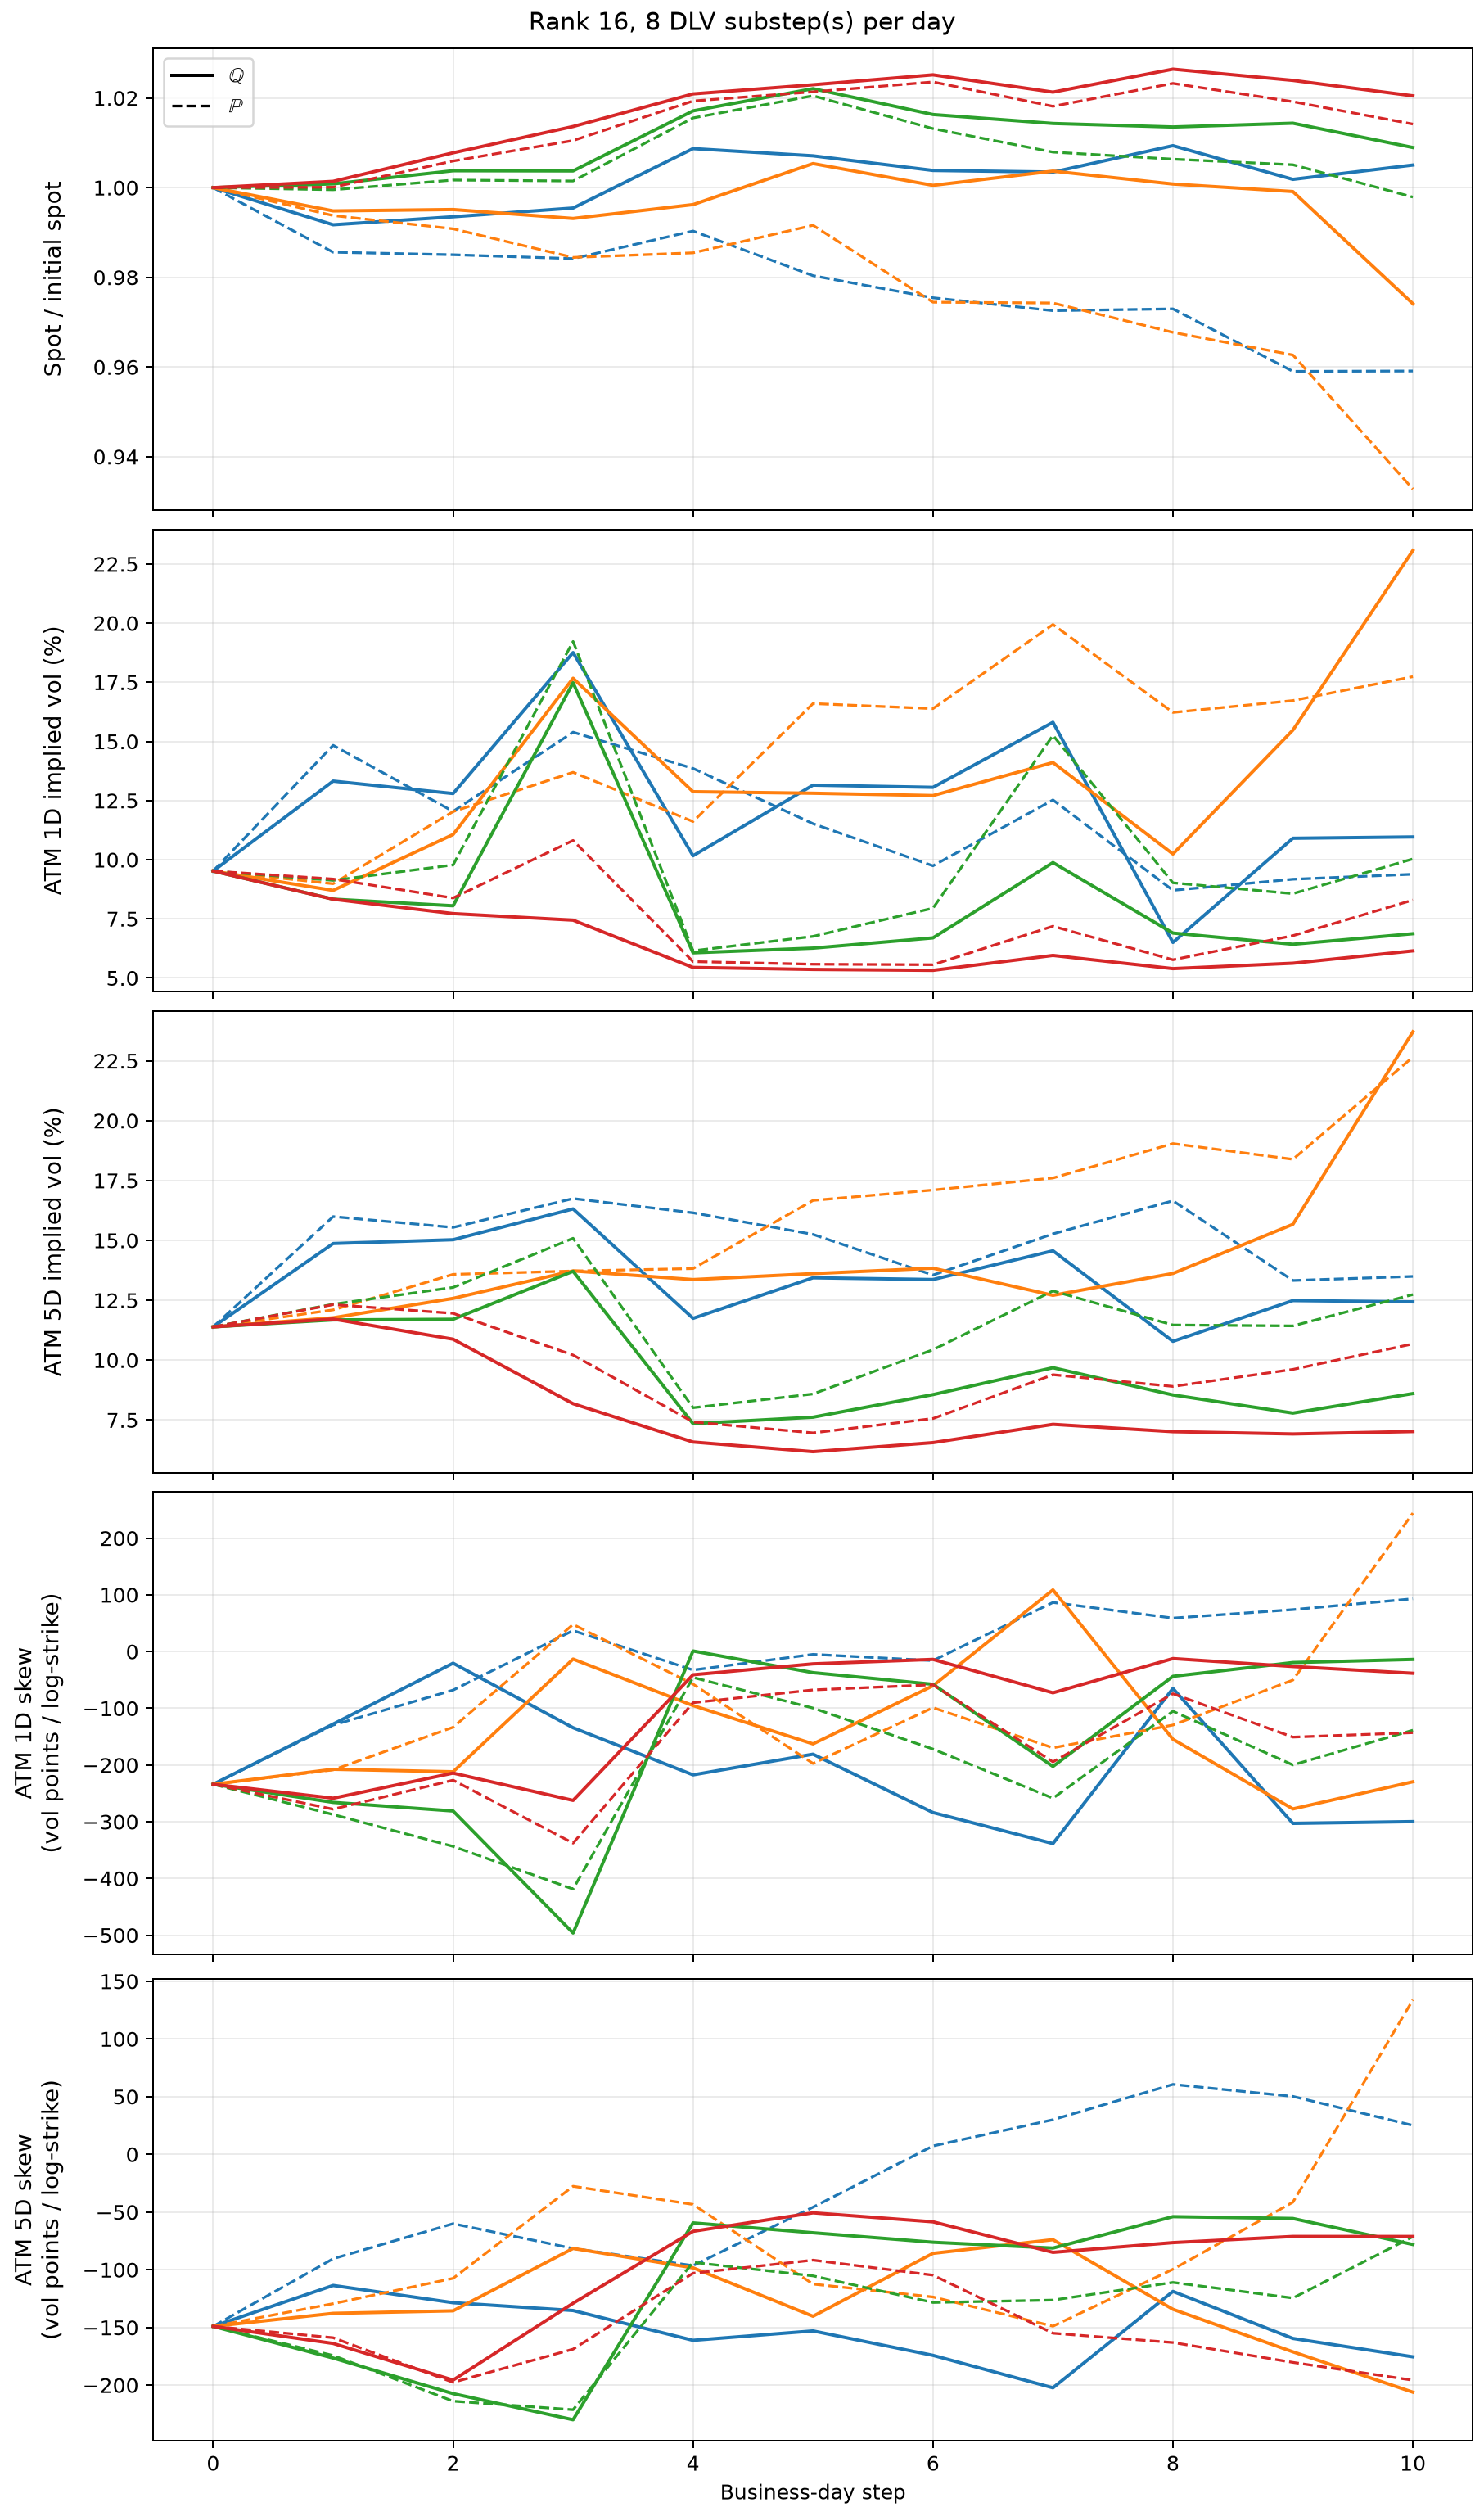
\includegraphics[height=0.88\textheight]
    {figures/front_spot/paths_rank16_eight_step.png}
  \caption{Matched $\PP/\Q$ paths for Model~D: rank 16 with eight Brownian
  substeps per day.}
  \label{fig:numerics-best-paths}
\end{figure}

\subsection{PCA Summary}
\label{app:dlv-factor-figures}

The remaining figures visualize the factor systems estimated in
Section~\ref{sec:estimation-vol-of-vol}.  Figure~\ref{fig:numerics-baseline-iv-3d}
is the baseline risk-neutral implied-volatility surface used for all factor
illustrations.


\begin{figure}[H]
  \centering
  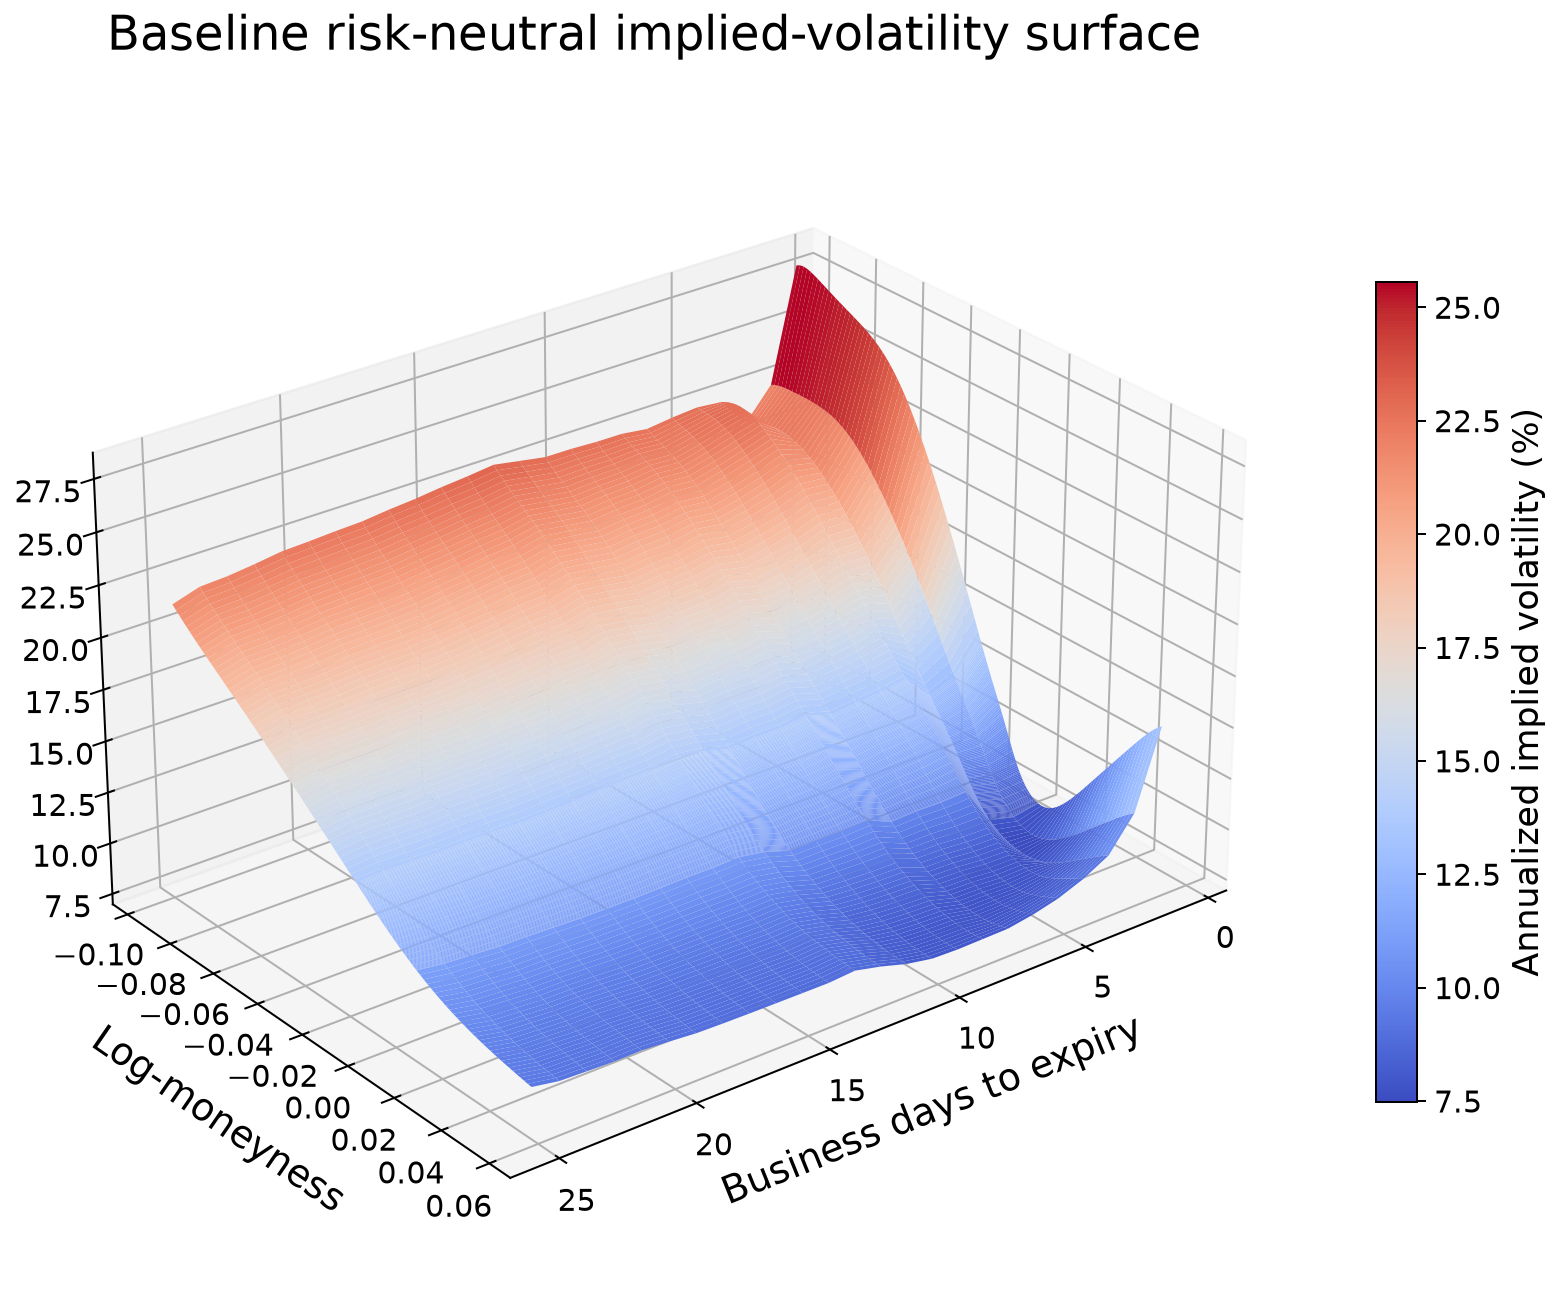
\includegraphics[width=0.72\textwidth]
    {figures/front_spot/baseline_implied_volatility_3d.png}
  \caption{Baseline annualized implied volatility on the fitted
  log-moneyness and business-days-to-expiry grid.}
  \label{fig:numerics-baseline-iv-3d}
\end{figure}

Figure~\ref{fig:numerics-factor-power} reports individual and cumulative PCA
power.  The experiments retain either eight or 16 factors; the first rank
above 90\% is 26.

\begin{figure}[H]
  \centering
  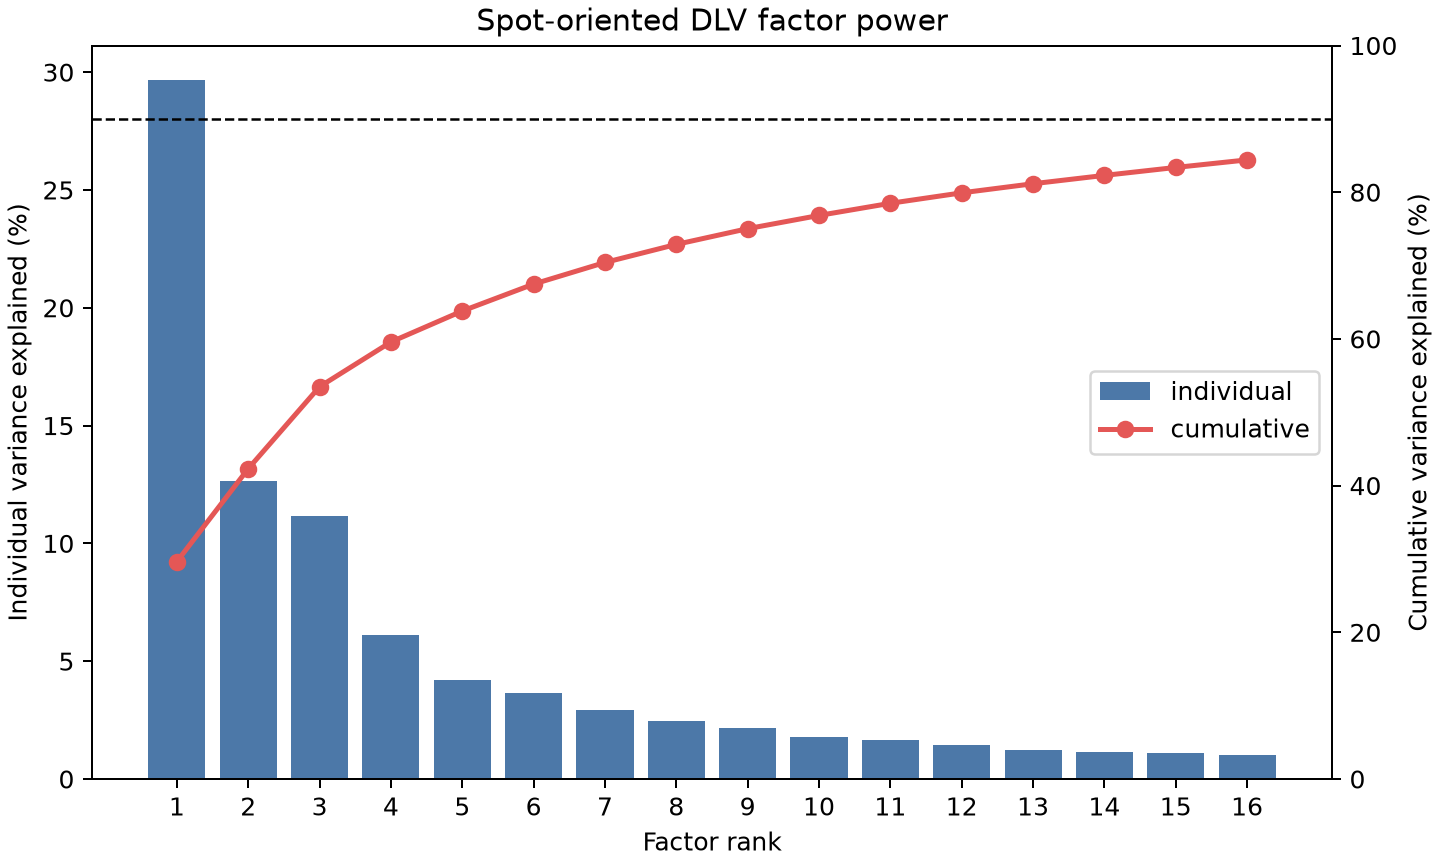
\includegraphics[width=0.88\textwidth]
    {figures/front_spot/pca_explained_variance.png}
  \caption{Individual and cumulative variance explained by the spot-oriented
  DLV factor system.  The vertical line is the rank-16 model cap; 26 factors
  are required to exceed 90\%.}
  \label{fig:numerics-factor-power}
\end{figure}

The rank-16 fit appends PCs 9--16 to the rank-8 fit.  A one-standard-deviation
shock is the diffusion-only log-DLV displacement
$\pm\xi_f\sqrt{1/252}$.  The figures display its central implied-volatility
response
\begin{equation}
  \label{eq:numerics-iv-factor-shock}
  \frac12\left[
    \sigma_{\mathrm{imp}}(\log\Sigma+\xi_f/\sqrt{252})
    -\sigma_{\mathrm{imp}}(\log\Sigma-\xi_f/\sqrt{252})
  \right].
\end{equation}
These shock directions are the same under $\PP$ and $\Q$: an equivalent
measure change alters drift, not diffusion.  Each panel deliberately retains
its own vertical scale.

\begin{figure}[H]
  \centering
  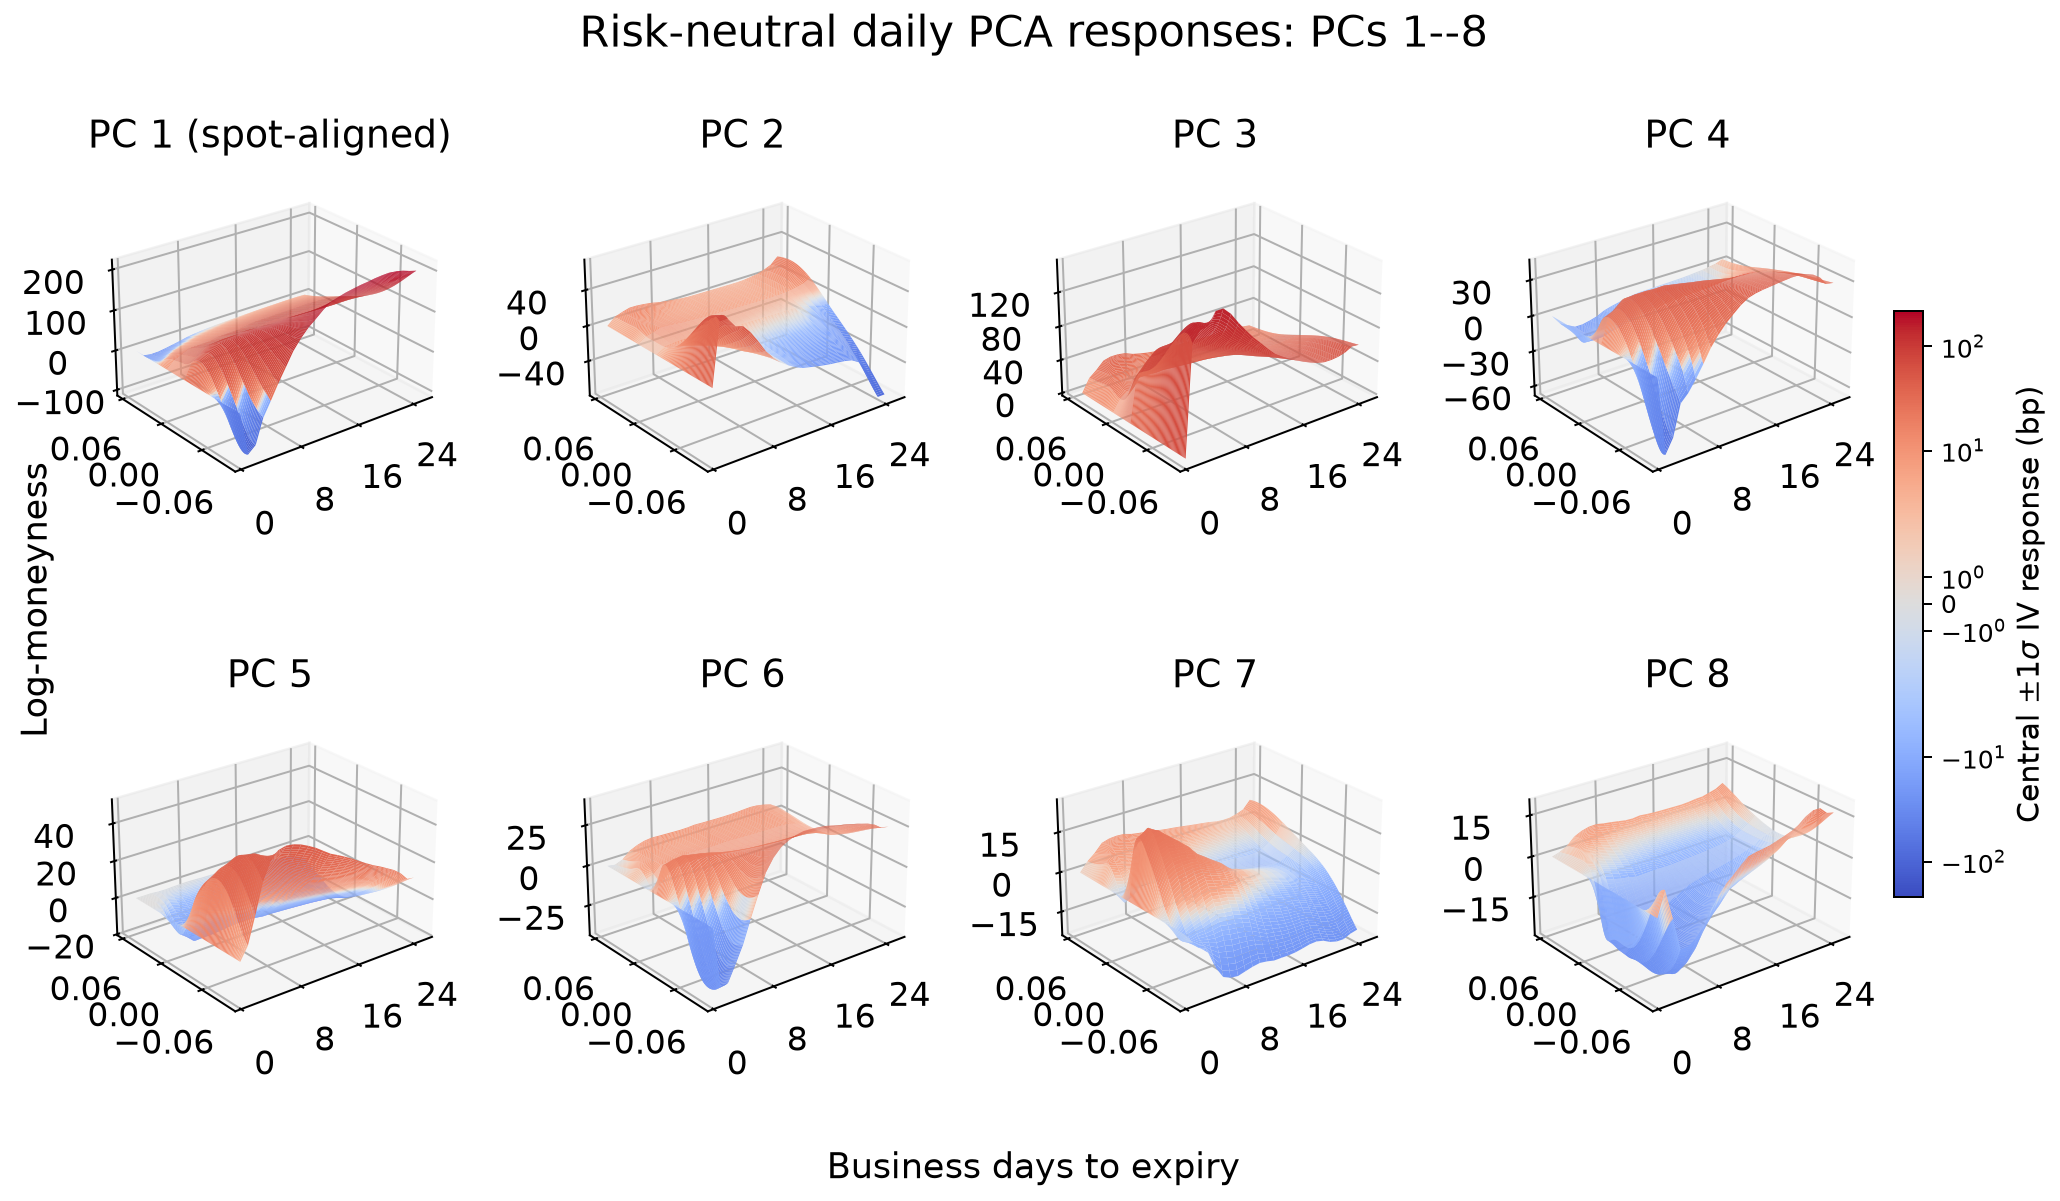
\includegraphics[width=\textwidth]
    {figures/front_spot/pca_factor_responses_3d_pc1_8.png}
  \caption{Risk-neutral one-standard-deviation implied-volatility responses
  for PCs 1--8.  PC~1 is aligned to the front-spot score.}
  \label{fig:numerics-pc1-8}
\end{figure}

\begin{figure}[H]
  \centering
  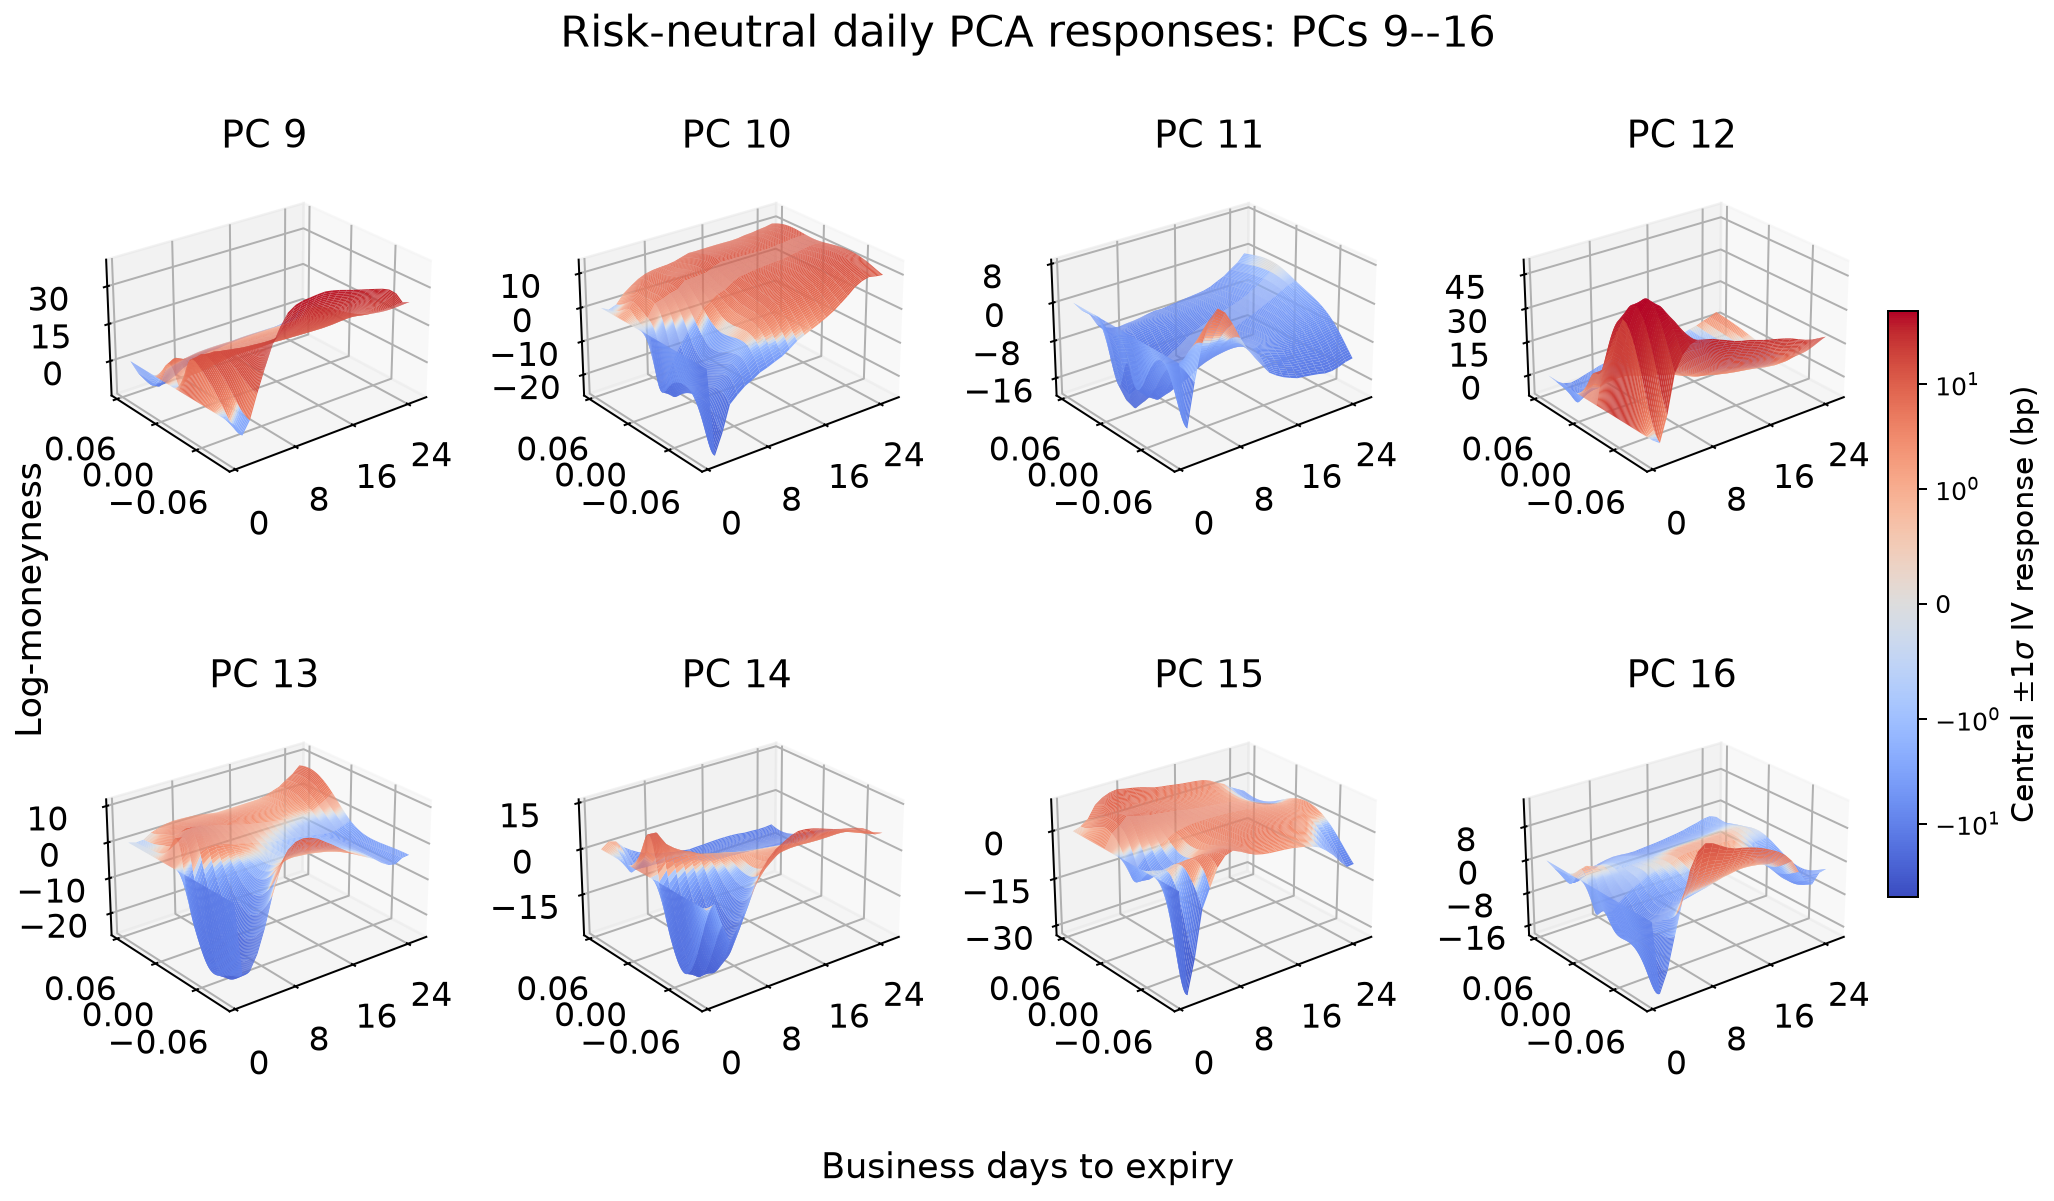
\includegraphics[width=\textwidth]
    {figures/front_spot/pca_factor_responses_3d_pc9_16.png}
  \caption{The additional one-standard-deviation implied-volatility responses,
  PCs 9--16, in the nested rank-16 model.}
  \label{fig:numerics-pc9-16}
\end{figure}

% !TEX root = main2.tex
\section{Market-data and calibration pipeline}
\label{app:market-pipeline}

This appendix records the data and numerical pipeline behind
Section~\ref{sec:estimation}. It follows the broader SPX pipeline described in
\cite{DYSANOS2026}, restricted here to the short-dated fixed-expiry SANOS
experiment. The complete transformation is
\[
\begin{aligned}
\text{raw IvyDB quotes}
&\longrightarrow \text{daily cleaning and parity-forward enrichment}\\
&\longrightarrow \text{arbitrage-free SANOS eligibility surface}\\
&\longrightarrow \text{European short-horizon quote selection}\\
&\longrightarrow \text{daily 25-by-200 calibration tensor}\\
&\longrightarrow \text{direct or affine end-to-end fit}.
\end{aligned}
\]

\subsection{Raw data and cleaning}
\label{app:pipeline-raw}

The source is OptionMetrics IvyDB US data accessed through WRDS. For each
eligible SPX market date we load the index level and previous index level,
option strikes and calendar expiries, call and put bid and ask quotes, volume,
open interest, AM/PM settlement flags, and the zero curve. The retained sample
runs from 3 January 2022 through 29 August 2025 and contains 891 valid full-day
NYSE sessions.

The raw cleaning step removes known bad ticker--date observations, missing or
invalid quotes, invalid settlement flags, same-day expiries, irregular
expiries, and quotes whose bid does not exceed $0.011$. Business days and year
fractions to expiry are then computed; an AM-settled expiry is treated as
$0.2$ of a business day earlier than its corresponding PM expiry.

For each expiry we recompute the forward from put--call parity rather than use
the delayed IvyDB forward table. With discount factor $D$, define the
discounted-forward bounds at a strike $K$ by
\[
  G^{\mathrm{ask}}(K)=C^{\mathrm{ask}}(K)-P^{\mathrm{bid}}(K)+DK,
  \qquad
  G^{\mathrm{bid}}(K)=C^{\mathrm{bid}}(K)-P^{\mathrm{ask}}(K)+DK.
\]
Their midpoint is averaged across strikes with inverse-spread weights,
\[
  \widehat G
  =\frac{\sum_K w_K\,[G^{\mathrm{ask}}(K)+G^{\mathrm{bid}}(K)]/2}
         {\sum_K w_K},
  \qquad
  w_K=\frac1{\max\{G^{\mathrm{ask}}(K)-G^{\mathrm{bid}}(K),10^{-3}\}}.
\]
The resulting forward is used to construct the tightest call-equivalent quote,
forward-normalized strikes and prices, implied volatilities, and Greeks. An
expiry must contain at least ten strikes with a traded call or put and at least
four strikes with both sides traded. The normalized spread must exceed
$10^{-6}$ and retained implied volatilities must lie between $0.01$ and $5$.

\subsection{Static preprocessing and quote selection}
\label{app:pipeline-static}

Before applying the model-specific horizon, the pipeline retains quotes with
vega per unit total volatility of at least $10^{-3}$, log volume and log open
interest of at least one, and at least ten surviving options per expiry. The
nominal per-day quote cap is 100,000 and is therefore non-binding here.

For data-quality control and to construct a stable ATM curve, every daily book
is passed through the linear SANOS preprocessing of \cite{SANOS2026}. The
strike grid is extended, each expiry is fitted inside the quoted bid--ask
intervals, negligible-density redundant strikes are removed, and the joint
surface fit enforces both butterfly and calendar-spread constraints. The
smoothness parameter is $0.25$. Expiries and strikes for which this
arbitrage-free auxiliary fit is unavailable are not passed to the final
calibration.

This auxiliary SANOS surface determines eligibility, the ATM term structure,
and the floating model support. It is not the calibration target: the JAX fits
in Section~\ref{sec:estimation-fit} use the original retained call and put
bid--ask intervals. No linear-programming state or fitted midpoint is supplied
as a target.

The final selection keeps European quotes no farther than 25 business days
from the observation date, excludes the $0.2$-business-day slice, and retains
the standardized log-moneyness interval $[-2.5,1.5]$. This leaves 2,192,458
quotes, between 1,590 and 5,096 per date.

\subsection{Daily calibration tensor}
\label{app:pipeline-tensor}

The model expiry grid is
\[
  T_j=\frac{j}{252},\qquad j=1,\ldots,25.
\]
For each date, 100 interior-strike candidates are generated from the front
ATM scale and 100 from the 25-day ATM scale. They are merged with a minimum
log-spacing safeguard to form one 200-node support shared across all model
expiries on that date. The support floats from date to date. Two boundary
nodes, equal to one half of the lowest inner strike and one and a half times
the highest inner strike, complete the 202-node density grid.

Each retained market quote stores its call/put flag, normalized strike, bid,
ask, midpoint, business days to expiry, adjacent model-expiry indices, and
linear interpolation weight. The contemporaneous SPX level is retained as a
reference spot. The immutable calibration tensor pads each date to a multiple
of 128 quotes and carries a Boolean mask, so padding never contributes to the
objective.

At valuation time the DLV recursion produces the 25 discrete densities. The
fixed 5\% Black factor convolves each discrete density into a smooth call-price
curve, and the two adjacent expiry curves are linearly interpolated to the
market quote's exact expiry. Puts follow from put--call parity.

\subsection{Optimization and retained artifacts}
\label{app:pipeline-optimization}

The direct and affine parameterizations are those in
Section~\ref{sec:estimation-fit}. Direct states are initialized from the
date-specific ATM term structure and are constant across strike at
initialization. Affine means use the average of these initial states; codes and
loadings receive small centered Gaussian initial values. DLV squared is bounded
between $10^{-4}$ and $9$, with a differentiable barrier near the upper bound.

The loss in \eqref{eq:estimation-quote-objective} is differentiated over every
retained quote. Quote blocks of size 128 are used only to limit accelerator
memory: their gradients are summed before each Adam update, so this is an exact
full-sample gradient rather than stochastic minibatching. Each fit uses 300
initial epochs with a cosine learning-rate schedule from $2\times10^{-2}$ to
$10^{-3}$, followed by a 700-epoch continuation from $5\times10^{-3}$ to
$5\times10^{-5}$. Checkpoints store either all daily direct states or the
affine mean, loadings, and daily codes. The retained reports recompute every
quote from the final checkpoint and produce the statistics in
Table~\ref{tab:numerics-static-market-fit}.


\bibliographystyle{alpha}
\bibliography{refs}

\end{document}
